\chapter{Auswertung}
\label{cha:Auswertung}
Die in diesem Kapitel genannten Standardfehler des Mittelwertes ergeben sich nach
\begin{equation*}
  \label{eqn:MW-Fehler}
  \sigma(x) = \sqrt{\frac{1}{n(n-1)} \sum_i (x_i - \overline{x})^2}.
\end{equation*}
Daraus resultierende Unsicherheiten genügen der Gaußschen Fehlerfortpflanzung.
Die Fehlerrechnung wird in \textit{Python} unter Verwendung des Paketes \textit{uncertainties} \cite{uncertainties} durchgeführt.



\begin{figure}
    \centering
    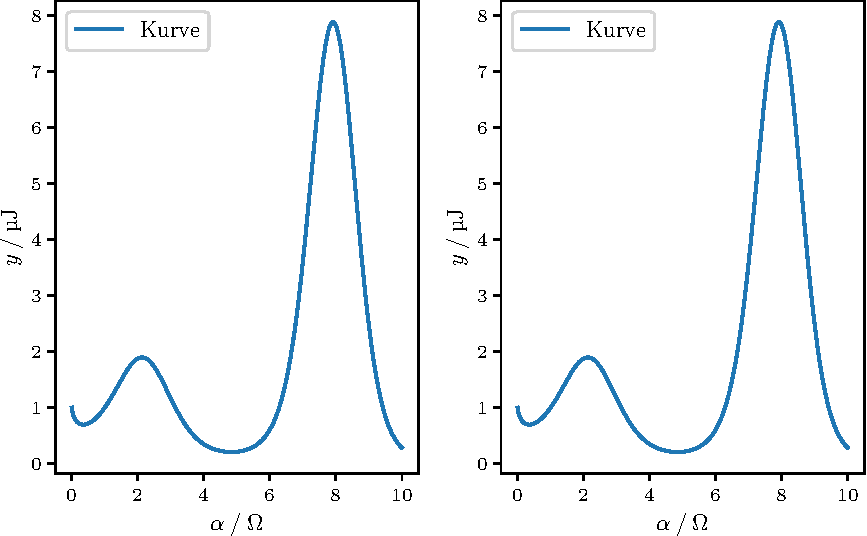
\includegraphics{plot.pdf}
    \caption{Plot.}
    \label{fig:plot}
\end{figure}